\documentclass[11pt]{article}
\usepackage{times}
\usepackage{latexsym}
\usepackage[T1]{fontenc}
\usepackage[utf8]{inputenc}
\usepackage{microtype}
\usepackage{acl}
\usepackage{booktabs}
\usepackage{graphicx}
\usepackage{amsmath,amssymb}
\usepackage{multirow}
\usepackage{tikz}
\usetikzlibrary{positioning,arrows.meta,fit,backgrounds}

\newcommand{\std}[1]{{\scriptsize$\pm$#1}}
\newcommand{\pihat}{\pi_\theta}
\newcommand{\RX}{RX-Hate}

\title{Hate Speech Detection through Explainable AI and Reward-Optimized Models:\\
A Multimodal, Code-Mixed Study with Faithful Rationales}

\author{[Author names]\\
Bennett University\\
\texttt{[author emails]}\\[2pt]
{\normalsize Supervisor: Dr.\ Pradeepika Verma (\texttt{pradeepika.verma@bennett.edu.in})}}

\begin{document}
\maketitle

\begin{abstract}
Hate speech detectors are usually text-only, trained on high-resource languages, and opaque. We study a
framework, \RX{}, for \emph{multimodal}, \emph{code-mixed} hate speech detection in which a policy outputs both a
label and the evidence for it, $\pihat(y,z\mid x)=\pihat(y\mid x)\,\pihat(z\mid x,y{=}1)$, for a post
$x=\{T,V,C\}$ made of text, image and context. After supervised warm-up, the policy is optimised with Group Relative Policy Optimisation (GRPO)
against a reward that mixes correctness, an identity-bias penalty, ERASER-style faithfulness, plausibility with
human rationales and conciseness, plus counterfactual logit pairing. Explanations are produced at token level
(learned rationale, Integrated Gradients, LIME, KernelSHAP) and at modality level (exact Shapley values over text, image and
context). Because no multimodal, code-mixed benchmark with exact ground truth for modality dependence exists, we build
\textsc{SynHateMM}, a HateCheck-style synthetic benchmark of 9{,}000 posts in English, Hinglish and romanised Hindi with
gold rationales, held-out templates and identity-swapped counterfactuals. On it, GRPO improves macro-F1 over its supervised
initialisation (85.4 vs.\ 83.5 macro-F1; better in all 3 seeds), cuts the counterfactual prediction gap from 5.8 to 2.4 points,
and \emph{lowers} agreement with human rationales (token-F1 82.9 vs.\ 90.2). Ablations show that counterfactual pairing
drives the accuracy and bias gains, that the faithfulness reward raises comprehensiveness in every seed (though GRPO's gain over SFT is
seed-dependent), and that the plausibility reward has no measurable effect. An early-fusion
logistic regression matches \RX{} on overall F1, so the benefit lies in bias sensitivity and explanations, not raw accuracy. All results are
on synthetic data and should be confirmed on real corpora; code for doing so, including an LLM (Qwen2.5 + LoRA, TRL) instantiation of the same rewards, is released.
\end{abstract}

%% ---------------------------------------------------------------------------------------------
\section{Introduction}
The growth of social media has amplified hate speech, with serious psychological and social consequences. Automatic
detectors help moderators cope with volume, but three gaps limit their use in sensitive settings such as moderation
and public-safety monitoring. (i)~Most systems are text-only and English-centric, whereas real posts mix languages and
scripts (``Hinglish''), use spelling variation and obfuscation, and are frequently hateful only in combination with an image or the
conversation they reply to \citep{kiela2020hateful,gomez2020mmhs,bohra2018hinglish}. (ii)~Neural and LLM detectors are black boxes whose
decisions moderators cannot audit. (iii)~Classifiers pick up spurious lexical cues and over-flag benign mentions of
identity groups, which hurts the very communities they should protect \citep{dixon2018bias,sap2019risk}.

We study a framework that addresses the three gaps together. Treating moderation as a decision with evidence, a policy
emits a label \emph{and} a token-level rationale, and is trained in two stages: supervised learning on the few
posts that carry human rationales, followed by reward optimisation with GRPO \citep{shao2024deepseekmath}. The reward encodes what
a trustworthy moderator should do: be correct, not flag benign identity mentions, and give rationales that are
\emph{faithful} (removing them changes the decision), \emph{plausible} (close to human ones) and \emph{concise}.

\paragraph{Contributions.}
(1)~A formulation of explainable hate detection as reward optimisation over $(y,z)$ pairs, with reward components
that are framework-agnostic and shared by a small fusion model and an LLM (Section~\ref{sec:method}).
(2)~\textsc{SynHateMM}, a synthetic multimodal, code-mixed benchmark with functional tests, gold rationales, counterfactuals and
held-out templates (Section~\ref{sec:data}).
(3)~An empirical study with three seeds, ablations and explainer comparisons (Section~\ref{sec:exp}), including negative results: the
plausibility reward adds nothing, optimising faithfulness trades away agreement with human rationales, and the faithfulness gain over SFT is not stable across seeds.
(4)~Open-source code covering the full pipeline, loaders for HateXplain, HASOC and Hateful Memes, and a GPU path for LLM GRPO.

\paragraph{Scope of the claims.}
Every number in this paper is measured on \textsc{SynHateMM} with a small NumPy model and hand-crafted image features.
We did not evaluate on real corpora or run the LLM path (the experimental environment had neither network access nor a GPU).
The results therefore show that the method behaves as designed under exact ground truth, and not how it ranks against
state-of-the-art systems on real data.

%% ---------------------------------------------------------------------------------------------
\section{Related Work}
\paragraph{Hate speech detection.}
Surveys document the progress and the difficulty of the task \citep{schmidt2017survey,fortuna2018survey}. Lexical
classifiers confuse offensive language with hate \citep{davidson2017automated}; HateCheck probes models with
functional tests such as counter-speech and non-protected targets \citep{rottger2021hatecheck}, a design we follow.
Multimodal benchmarks include MMHS150K \citep{gomez2020mmhs} and Hateful Memes \citep{kiela2020hateful}, whose
confounders flip a label by changing one modality. Indo-European and code-mixed resources include HASOC \citep{mandl2019hasoc}
and Hinglish corpora \citep{bohra2018hinglish}; multilingual encoders \citep{conneau2020xlmr,khanuja2021muril} are the usual
route to low-resource transfer.

\paragraph{Explainability.}
HateXplain adds human token rationales to hate data \citep{mathew2021hatexplain}. Post-hoc attribution uses
gradients \citep{sundararajan2017ig}, local surrogates \citep{ribeiro2016lime} or Shapley values \citep{lundberg2017shap,shapley1953value};
self-explaining models learn rationales jointly \citep{lei2016rationalizing}. ERASER defines plausibility and faithfulness via
comprehensiveness and sufficiency \citep{deyoung2020eraser}, and \citet{jacovi2020faithfulness} caution against conflating the two.

\paragraph{Fairness.}
Identity-term bias is measured with subgroup, BPSN and BNSP AUC \citep{borkan2019nuanced}, equality differences
\citep{dixon2018bias} and counterfactual token fairness \citep{garg2019counterfactual}.

\paragraph{Reward optimisation.}
RLHF \citep{ouyang2022instructgpt} and its variants optimise models against a learned or programmatic reward; GRPO replaces the value
function by a group-normalised advantage \citep{shao2024deepseekmath} on top of PPO's clipped objective \citep{schulman2017ppo}. We use
programmatic rewards (no learned reward model), which makes every term inspectable.

%% ---------------------------------------------------------------------------------------------
\section{Method}\label{sec:method}
\subsection{Problem formulation}
A post is $x_i=\{T_i,V_i,C_i\}$: text $T_i$ (possibly multilingual or code-mixed), visual content $V_i$ (image or meme) and
context $C_i$ (parent post, community, thread toxicity). Detection learns $f_\theta(x_i)\to y_i\in\{0,1\}$ (non-hateful / hateful).
We extend the prediction with a rationale $z_i\in\{0,1\}^{|T_i|}$ marking the tokens that justify a hateful decision. The
\emph{action} of the policy is $a=(y,z)$ with
\begin{equation}
\pihat(y,z\mid x)=\pihat(y\mid x)\prod_{t}\pihat(z_t\mid x,y{=}1)^{[y=1]},
\end{equation}
i.e.\ a non-hateful decision carries the empty rationale.

\subsection{Fusion policy}
Figure~\ref{fig:overview} sketches the model. Text is normalised for code-mixed input (lower-casing, de-leetspeak, squeezing of
elongations, mapping of common romanised-Hindi spelling variants) and encoded with signed feature hashing
\citep{weinberger2009hashing} of word uni- and bi-grams and within-word character 2--4-grams, which needs no vocabulary and degrades
gracefully on spelling variation. Images are described by colour histograms, HOG-style gradient histograms and spatial colour layout
(a frozen CLIP encoder \citep{radford2021clip} is the intended drop-in). The context encoder embeds the parent post and metadata. Three ReLU encoders
($h_T,h_V,h_C$) feed a late-fusion layer and a softmax label head. The rationale head scores each token from the token and its
$\pm2$ neighbours, so the same word can be treated differently in ``\emph{X are vermin}'' and ``\emph{calling X vermin is wrong}''.
Modality dropout during training makes the ``absent modality'' state in-distribution, which the Shapley analysis relies on.

\begin{figure}[t]
\centering
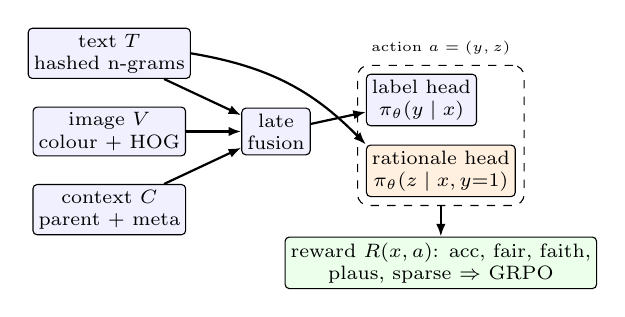
\begin{tikzpicture}[font=\scriptsize, node distance=3.5mm, every node/.style={align=center},
  box/.style={draw, rounded corners=1.5pt, minimum height=5mm, inner sep=2pt, fill=blue!6},
  rbox/.style={draw, rounded corners=1.5pt, minimum height=5mm, inner sep=2pt, fill=orange!12},
  arr/.style={-{Latex[length=1.6mm]}, thick}]
\node[box] (T) {text $T$\\hashed n-grams};
\node[box, below=of T] (V) {image $V$\\colour + HOG};
\node[box, below=of V] (C) {context $C$\\parent + meta};
\node[box, right=7mm of V] (F) {late\\fusion};
\node[box, right=7mm of F, yshift=4mm] (Y) {label head\\$\pihat(y\mid x)$};
\node[rbox, right=7mm of F, yshift=-5mm] (Z) {rationale head\\$\pihat(z\mid x,y{=}1)$};
\draw[arr] (T) -- (F); \draw[arr] (V) -- (F); \draw[arr] (C) -- (F);
\draw[arr] (F) -- (Y);
\draw[arr] (T.east) to[bend left=18] (Z.north west);
\node[draw, dashed, rounded corners, fit=(Y)(Z), inner sep=3pt, label={[font=\tiny]above:action $a=(y,z)$}] (A) {};
\node[draw, fill=green!8, rounded corners=1.5pt, below=5mm of Z, minimum height=5mm, inner sep=2pt] (R)
 {reward $R(x,a)$: acc, fair, faith,\\plaus, sparse $\Rightarrow$ GRPO};
\draw[arr] (A.south) -- (R.north);
\end{tikzpicture}
\caption{Overview of \RX{}. The policy acts with a label and a rationale; the reward scores both.}
\label{fig:overview}
\end{figure}

\subsection{Rewards}\label{sec:reward}
For an action $a=(\hat y,z)$ on a post with gold label $y$, optional human rationale $z^\star$ and an identity mention flag $m$:
\begin{multline}
R=w_a r_{acc}+w_f r_{fair}+w_{\phi} r_{faith}\\+w_p r_{plaus}+w_s r_{sparse}+w_e r_{empty}.
\end{multline}
\textbf{Correctness} $r_{acc}=+1$ if $\hat y=y$, else $-1$ (the code supports asymmetric costs). \textbf{Fairness}
$r_{fair}=-1$ if $\hat y=1,\,y=0$ and $m=1$: flagging a benign post that mentions an identity group is the dominant source of unintended bias.
\textbf{Faithfulness} for $\hat y=1$ combines comprehensiveness and sufficiency \citep{deyoung2020eraser},
$r_{faith}=\big(p(x)-p(x\setminus z)\big)-\max\big(0,\,p(x)-p(z)\big)$, with $p$ the policy's own hate probability on
the post, on the post with the rationale removed and on the rationale alone; an empty rationale for a hateful decision receives $-1$.
\textbf{Plausibility} $r_{plaus}$ is the token-F1 of $z$ against $z^\star$ when the post has a human rationale. \textbf{Conciseness}
$r_{sparse}=-\max(0,\bar z-\rho)$ penalises rationales covering more than a fraction $\rho$ of the tokens, and $r_{empty}=-\bar z$ for $\hat y=0$.
Weights are $w_a{=}1$, $w_f{=}w_\phi{=}w_p{=}0.5$, $w_s{=}w_e{=}0.3$ and $\rho{=}0.6$ (the mean human-rationale
length in the training set); we did not tune them beyond a coarse check on the validation set.

\subsection{Optimisation}
\paragraph{Stage 1 (SFT).} Cross-entropy for the label plus binary cross-entropy for the rationale head on hateful posts
that carry human rationales, with modality dropout and early stopping on validation macro-F1.
\paragraph{Stage 2 (GRPO).} For each post we sample $G{=}8$ actions from the current policy, score them with $R$, and
use the group-normalised advantage $A_g=(R_g-\bar R)/(\sigma_R+\epsilon)$. The policy is updated with the clipped
surrogate and an exact KL penalty to the frozen SFT policy, plus \emph{counterfactual logit pairing} that penalises
$\big(\ell(x)-\ell(x^{cf})\big)^2$ between the hate logit of a post and of the same post with its identity term swapped
\citep{garg2019counterfactual}:
\begin{multline}
\mathcal L=-\mathbb E\big[\min(\rho_g A_g,\operatorname{clip}(\rho_g,1{\pm}\epsilon)A_g)\big]\\
+\beta\,\mathrm{KL}(\pihat\Vert\pi_{\mathrm{SFT}})+\lambda\big(\ell(x)-\ell(x^{cf})\big)^2 .
\end{multline}
We use $\epsilon{=}0.2$, $\beta{=}0.04$, $\lambda{=}0.5$, Adam with learning rate $5\cdot10^{-4}$, batches of 32 posts, two inner steps per rollout and three epochs;
the checkpoint with the best validation reward is kept. The network is implemented in NumPy with hand-derived back-propagation, which the test suite verifies against finite differences.

\subsection{Explanations}
Token level: (a)~the policy's \emph{learned rationale}; post-hoc (b)~Integrated Gradients (IG; zero baseline, 32 steps),
(c)~leave-one-out occlusion, (d)~LIME and (e)~KernelSHAP over token masks (300 samples). Modality level: exact Shapley values of the
hate logit over the three players \{text, image, context\}, where an absent player's input is zeroed. A report combines
the prediction, the rationale, the most influential words, per-modality contributions, the targeted identity terms and a note
when the decision is driven mainly by the image or context.

%% ---------------------------------------------------------------------------------------------
\section{The \textsc{SynHateMM} Benchmark}\label{sec:data}
Real multimodal, code-mixed hate corpora lack ground truth for \emph{why} a post is hateful, which prevents controlled measurement
of modality dependence and rationale quality. We therefore generate 9{,}000 posts (6{,}348 train / 837 validation / 1{,}815 test; 46--49\% hateful)
from templates, in the style of HateCheck \citep{rottger2021hatecheck}. Templates contain no slurs and the
``hate symbols'' in images are invented shapes.

\paragraph{Languages and noise.} 55\% English, 30\% Hinglish, 15\% romanised Hindi. Tokens receive Hinglish
spelling variants, leetspeak on abusive words, typos and filler tokens; 3\% of training labels are flipped.

\paragraph{Fourteen functionalities} (Table~\ref{tab:func}): six hateful (derogation, threat/exclusion, implicit, sarcastic, hate via
\emph{image}, hate via \emph{context}) and eight non-hateful, including neutral and positive identity mentions, \emph{counter-speech} that reuses
hateful vocabulary, abuse of non-protected targets, benign sarcasm, an educational post showing a hate symbol, and
two confounders. In the image and context confounders the text is \emph{identical} across labels, and only the image (or the parent post) decides.

\paragraph{Rationales, counterfactuals, generalisation.} Hateful posts carry gold token rationales (mean 59\% of tokens); only 30\% of training
posts expose them, mimicking scarce human annotation. Every post that mentions a group has an identity-swapped counterfactual. The
last template of every template list and the last lexicon item are never seen in training, and test posts use them with probability 0.5
(45\% of test posts use an unseen template), which separates memorisation from generalisation.

%% ---------------------------------------------------------------------------------------------
\section{Experiments}\label{sec:exp}
\paragraph{Setup.} Baselines: word and character TF-IDF logistic regression (text only) and an early-fusion logistic regression over all
modalities. The fusion policy is trained with 15 SFT epochs at most (early stopping) and 3 GRPO epochs, for three seeds (0--2); we report
mean$\pm$std over seeds, and single runs for the deterministic linear baselines. Metrics: accuracy, macro-F1, AUROC; per-functionality accuracy;
the bias metrics of Section~\ref{sec:method}; rationale plausibility (AUPRC, token-F1 and IoU-F1 against gold rationales on hateful test posts) and
faithfulness (comprehensiveness and sufficiency). The generalised-mean bias AUCs use power $-5$.
Everything ran on a 2-core CPU in about two hours.

\subsection{Main results}
\begin{table*}[t]
\centering\small\setlength{\tabcolsep}{3.6pt}
\begin{tabular}{lcccccccc}
\toprule
 & Acc & Macro-F1 & AUROC & F1 seen & F1 unseen & F1 en & F1 hi-en & F1 hi \\
\midrule
TF-IDF word + LR & 74.9 & 74.8 & 83.0 & 86.4 & 60.8 & 70.0 & 80.3 & 79.8 \\
TF-IDF char + LR & 78.8 & 78.7 & 85.2 & 87.7 & 68.0 & 74.0 & 82.1 & 87.5 \\
Early-fusion LR (T+V+C) & 85.3 & 85.2 & 88.6 & 96.8 & 71.3 & 82.5 & 86.9 & 91.6 \\
\midrule
Fusion SFT (T) & 74.4\std{0.9} & 74.4\std{0.9} & 84.8\std{1.5} & 86.7\std{0.7} & 59.1\std{2.6} & 69.1\std{1.6} & 78.3\std{2.3} & 85.0\std{2.1} \\
Fusion SFT (T+V) & 80.0\std{0.7} & 79.9\std{0.7} & 87.5\std{1.0} & 92.5\std{0.7} & 64.7\std{1.7} & 77.0\std{0.5} & 81.8\std{2.1} & 86.6\std{2.4} \\
Fusion SFT (T+V+C) & 83.6\std{0.7} & 83.5\std{0.6} & 89.1\std{0.5} & 97.5\std{0.3} & 66.6\std{1.6} & 79.5\std{0.6} & 86.8\std{2.5} & 90.6\std{3.7} \\
\midrule
\textbf{RX-Hate: SFT + GRPO (T+V+C)} & 85.5\std{0.3} & 85.4\std{0.3} & 90.0\std{0.6} & 98.3\std{0.5} & 69.9\std{0.5} & 82.1\std{0.6} & 87.4\std{1.4} & 92.9\std{1.9}
\\
\bottomrule
\end{tabular}
\caption{Test results on \textsc{SynHateMM} (\%). ``Seen/unseen'' split test posts by whether their template was in training.
Fusion models: mean$\pm$std over 3 seeds; linear baselines: single run.}
\label{tab:main}
\end{table*}

Table~\ref{tab:main} shows the pattern one expects from the benchmark's design. Text-only models are far worse than multimodal ones
(74.4 F1 for the text-only fusion policy). Adding the image and context gives +5.5 and +3.6 F1.
GRPO then improves the supervised policy from 83.5$\pm$0.6 to 85.4$\pm$0.3 F1 (in each seed: 85.7, 85.3, 85.1 against 83.9, 83.9, 82.6 for the same initialisations) and from 66.6 to 69.9 on unseen templates (better in all seeds). However, the early-fusion logistic regression reaches 85.2 F1 overall and
\emph{higher} F1 on unseen templates (71.3), so on pure classification \RX{} is on par with a strong linear baseline in this
synthetic setting. The advantage of the policy lies elsewhere: it is the only model that also produces rationales, and it is less sensitive to identity swaps than the supervised policy (Table~\ref{tab:fair}).
Performance on romanised Hindi is high for all models, probably because its templates share lexical items with the Hinglish ones (see the low-resource analysis below).

\begin{table*}[t]
\centering\small\setlength{\tabcolsep}{4pt}
\begin{tabular}{lcccccccc}
\toprule
Model & Sub-AUC$\uparrow$ & BPSN$\uparrow$ & BNSP$\uparrow$ & FPED$\downarrow$ & FNED$\downarrow$ & ID-FPR$\downarrow$ & CTF gap$\downarrow$ & Flip$\downarrow$\\
\midrule
TF-IDF char + LR & 81.9 & 81.2 & 85.9 & 0.70 & 0.54 & 23.9 & 3.3 & 3.9 \\
Early-fusion LR & 85.0 & 85.5 & 88.2 & 0.61 & 0.37 & 19.2 & 2.5 & 2.0 \\
Fusion SFT & 85.7\std{0.7} & 85.8\std{0.6} & 89.0\std{0.7} & 0.55\std{0.07} & 0.45\std{0.07} & 19.2\std{2.8} & 5.8\std{0.5} & 5.6\std{0.8} \\
\textbf{RX-Hate (GRPO)} & 86.5\std{0.8} & 87.1\std{0.7} & 89.7\std{0.7} & 0.48\std{0.07} & 0.27\std{0.02} & 17.9\std{0.9} & 2.4\std{0.2} & 2.2\std{0.2}
\\
\bottomrule
\end{tabular}
\caption{Unintended-bias metrics (\%, except FPED/FNED). BPSN/BNSP: background-positive/negative subgroup-negative/positive AUC
(generalised mean over 11 identity groups); FPED/FNED: false-positive/negative equality difference; ID-FPR: false-positive rate on non-hateful posts mentioning a group;
CTF gap: mean $|p(x)-p(x^{cf})|$ after swapping the identity term; Flip: fraction of decisions that flip.}
\label{tab:fair}
\end{table*}

\subsection{Functional tests}
\begin{table*}[t]
\centering\small\setlength{\tabcolsep}{4pt}
\begin{tabular}{lccccccc}
\toprule
Functionality & Label & $n$ & Char LR & EF-LR & SFT (T) & SFT & GRPO \\
\midrule
Derogation & H & 223 & \textbf{100.0} & 97.3 & 99.4 & 93.1 & 95.8 \\
Threat / exclusion & H & 173 & \textbf{68.2} & 61.3 & 64.5 & 60.7 & 62.8 \\
Implicit / coded & H & 147 & \textbf{100.0} & 89.8 & 85.9 & 78.2 & 83.9 \\
Sarcastic hate & H & 75 & 69.3 & 70.7 & 69.8 & 72.4 & \textbf{73.3} \\
Hate via image & H & 136 & 53.7 & 88.2 & 67.2 & 96.1 & \textbf{99.5} \\
Hate via context & H & 84 & 45.2 & \textbf{92.9} & 57.9 & 80.2 & 87.3 \\
\midrule
Neutral identity mention & N & 159 & \textbf{98.7} & 96.9 & 92.2 & 96.0 & 98.3 \\
Positive statement & N & 136 & 79.4 & 80.9 & 70.8 & 81.6 & \textbf{82.4} \\
Counter-speech & N & 150 & \textbf{72.7} & 70.0 & 65.3 & 67.1 & 66.9 \\
Abuse, non-protected & N & 133 & \textbf{99.2} & 93.2 & 93.7 & 94.7 & 95.2 \\
Benign sarcasm & N & 61 & \textbf{100.0} & 98.4 & \textbf{100.0} & 97.3 & 96.2 \\
Benign image (confounder) & N & 128 & 48.4 & 73.4 & 30.2 & 77.1 & \textbf{79.4} \\
Educational symbol post & N & 93 & \textbf{100.0} & 90.3 & 99.3 & 86.4 & 81.0 \\
Benign context (confounder) & N & 117 & 49.6 & \textbf{94.9} & 35.0 & 92.9 & 94.6
\\
\bottomrule
\end{tabular}
\caption{Accuracy (\%) per functionality; bold marks the best. EF-LR: early-fusion LR; SFT (T): text-only fusion policy.}
\label{tab:func}
\end{table*}
Table~\ref{tab:func} shows where models fail. Text-only models score at or below chance on the image and context confounders (30--67\%; the text is identical
across labels), the multimodal ones 73--99\%, and GRPO gives the best result on hate-via-image (99.5) and benign-image (79.4). Counter-speech is hard for all models
(65.3--72.7\%), presumably because hateful vocabulary inside a condemnation looks like hate. Threat/exclusion posts are the weakest of the textual hateful classes (60.7--68.2\%; GRPO 62.8), partly because
half of the test threats use unseen templates. The character-n-gram baseline reaches 99--100\% on several
text-only functionalities but fails on exactly the cases that require the other modalities.

\subsection{Fairness}
GRPO improves on the supervised policy on every metric in Table~\ref{tab:fair}. The counterfactual gap falls from 5.8 to 2.4 points (lower in each seed: 2.1, 2.6, 2.5 vs.\ 5.2, 6.2, 6.1),
the flip rate from 5.6 to 2.2\%, FPED from 0.55 to 0.48 and the false-positive rate on benign identity mentions from 19.2 to 17.9\%. The last change is small and driven by one seed (per-seed ID-FPR 16.8, 18.2, 18.8 vs.\ 16.2, 18.5, 22.9).
The early-fusion LR has a similar counterfactual gap (2.5) and flip rate (2.0), with higher FPED (0.61) and ID-FPR (19.2). The ID-FPR remains high in absolute terms (about 18\%): in the three GRPO runs, the false positives on posts that
mention a group come mostly from counter-speech (47--53 of 150 posts flagged), benign-image posts (25--28 of 128) and positive statements (21--27 of 136).

\subsection{Ablations}
\begin{table*}[t]
\centering\small\setlength{\tabcolsep}{3.4pt}
\begin{tabular}{lcccccccc}
\toprule
Variant & F1 & F1 unseen & BPSN & ID-FPR & CTF gap & Tok-F1 & Comp. & Suff.\\
\midrule
SFT only & 83.5\std{0.6} & 66.6\std{1.6} & 85.8\std{0.6} & 19.2\std{2.8} & 5.8\std{0.5} & 90.2\std{0.5} & 16.7\std{2.7} & 6.0\std{0.6} \\
\midrule
\textbf{Full RX-Hate (GRPO)} & 85.4\std{0.3} & 69.9\std{0.5} & 87.1\std{0.7} & 17.9\std{0.9} & 2.4\std{0.2} & 82.9\std{2.4} & 21.2\std{7.9} & 3.9\std{2.0} \\
\midrule
$-$ fairness reward & 85.0\std{0.2} & 69.1\std{0.6} & 87.2\std{0.5} & 19.4\std{1.6} & 2.8\std{0.6} & 84.2\std{3.9} & 18.4\std{8.1} & 3.6\std{2.0} \\
$-$ faithfulness reward & 85.0\std{0.7} & 69.4\std{0.6} & 87.1\std{0.6} & 16.7\std{0.9} & 2.9\std{0.3} & 86.8\std{2.1} & 12.9\std{3.3} & 6.2\std{0.4} \\
$-$ plausibility reward & 84.9\std{0.5} & 69.1\std{0.6} & 86.9\std{0.5} & 18.6\std{0.9} & 2.5\std{0.2} & 83.0\std{2.3} & 21.9\std{7.7} & 3.7\std{2.3} \\
$-$ counterfactual pairing & 83.3\std{0.4} & 66.7\std{1.2} & 85.6\std{1.0} & 21.5\std{0.9} & 5.6\std{0.5} & 84.0\std{1.7} & 24.9\std{6.0} & 4.3\std{1.5} \\
$-$ KL to reference & 85.1\std{0.6} & 69.6\std{1.1} & 87.4\std{0.9} & 18.0\std{0.9} & 2.8\std{0.6} & 84.4\std{3.6} & 18.7\std{8.2} & 4.2\std{1.8} \\
REINFORCE (no group norm.) & 84.7\std{0.3} & 68.8\std{0.6} & 87.0\std{0.5} & 17.7\std{1.2} & 3.2\std{0.3} & 88.9\std{1.5} & 13.6\std{3.7} & 5.6\std{0.5}
\\
\bottomrule
\end{tabular}
\caption{Ablations (\%; 3 seeds). Tok-F1: token-F1 with gold rationales (plausibility); Comp./Suff.: comprehensiveness (higher is better) and
sufficiency gap (lower is better), measured with the policy itself on the hard rationale mask.}
\label{tab:abl}
\end{table*}
Table~\ref{tab:abl} removes one component at a time. \textbf{Counterfactual pairing} is the most important component for accuracy and fairness: without it F1 drops to 83.3 (2.1 below
the full model) and the counterfactual gap rises from 2.4 to 5.6, i.e.\ back to the SFT level, so GRPO's bias gains come
from the pairing term and not from the reward alone. \textbf{Faithfulness} reward raises comprehensiveness from 12.9 to 21.2 and lowers the sufficiency gap
from 6.2 to 3.9, at the cost of agreement with human rationales (86.8 to 82.9 token-F1). The comprehensiveness gain is positive in each seed (per-seed full vs.\ ablated: 18.7/13.0/31.9 vs.\ 13.4/8.6/16.6)
but the size varies strongly ($\pm$7.9). \textbf{Plausibility} reward has no measurable effect (token-F1 83.0 without it vs.\ 82.9 with it), probably because the SFT warm-up already supplies the
supervision and the noisy RL signal adds nothing. The \textbf{fairness} reward lowers ID-FPR from 19.4 to 17.9, a change comparable to the seed std.\ (1.6/0.9). Group normalisation
beats plain REINFORCE with a moving baseline (+0.7 F1, comprehensiveness 21.2 vs.\ 13.6), and removing the KL term has no clear effect at this training length. Removing counterfactual pairing
\emph{increases} comprehensiveness (24.9), so the bias term and the faithfulness term compete to some degree.

\paragraph{Plausibility--faithfulness trade-off.} SFT gives the highest plausibility (token-F1 90.2, lower for GRPO in every seed) and the lowest sufficiency-based faithfulness (gap 6.0 vs.\ 3.9; comprehensiveness 16.7 vs.\ 21.2, though per seed GRPO is
better only in seed 2: 31.9 vs.\ 16.6, with 18.7 vs.\ 20.0 and 13.0 vs.\ 13.4 in the others). GRPO's rationales are
longer (69.5\% of tokens vs.\ 57.7\% for SFT and 58.4\% for humans) and less human-like. This is the tension \citet{jacovi2020faithfulness} describe: rationales that look
right to people need not be those that drive the model. We therefore regard the faithfulness gain over SFT as suggestive, not established.

\subsection{Explanation methods}
\begin{table*}[t]
\centering\small\setlength{\tabcolsep}{3.4pt}
\begin{tabular}{lccccc|ccc}
\toprule
& \multicolumn{5}{c|}{GRPO policy} & \multicolumn{2}{c}{SFT policy} & \\
Method & AUPRC & Tok-F1 & IoU-F1 & Comp.$\uparrow$ & Suff.$\downarrow$ & Tok-F1 & Comp. & ms/post\\
\midrule
Integrated Gradients & 70.3 & 59.5 & 43.5 & 25.8 & -2.7 & 58.3 & 33.2 & 12 \\
Occlusion & 67.6 & 56.6 & 38.8 & 25.5 & -2.5 & 56.9 & 33.1 & 2 \\
LIME & 68.1 & 58.6 & 39.6 & 26.5 & -2.9 & 58.3 & 34.4 & 14 \\
KernelSHAP & 68.9 & 58.8 & 41.9 & 26.1 & -3.2 & 58.5 & 33.7 & 17 \\
\textbf{Learned rationale (ours)} & 96.7 & 76.9 & 81.2 & 11.1 & 7.6 & 77.9 & 13.4 & 2 \\
Random & 66.4 & 56.9 & 44.2 & 5.2 & 16.2 & 56.2 & 8.1 & 1
\\
\bottomrule
\end{tabular}
\caption{Token-level explainers on 300 hateful test posts that the policy flags correctly (\%). Hard masks keep the top-$k$ tokens with $k$ equal to the mean gold rationale length (58\%);
faithfulness is averaged over top-10/20/30/50\% masks. Learned-rationale Tok-F1 here uses the fixed-$k$ protocol, so it differs from Table~\ref{tab:abl}, which thresholds at 0.5.}
\label{tab:xai}
\end{table*}
Table~\ref{tab:xai} compares explainers on the same policy. The learned rationale is by far the most plausible (AUPRC 96.7 vs.\ 68--70 for post-hoc methods and 66.4 for random; token-F1 76.9 vs.\ 57--60)
and cheap (2\,ms/post, like occlusion, vs.\ 12--17\,ms for IG, LIME and KernelSHAP). Post-hoc methods, however, rank higher on comprehensiveness (25.5--26.5 vs.\ 11.1) and sufficiency (negative values, i.e.\ better than the full post) than the learned rationale (7.6),
so they are \emph{more faithful by the ERASER measure}. Their plausibility is close to random (AUPRC 68--70 vs.\ 66; IoU-F1 below random), consistent with the model relying partly on tokens that annotators did not mark (we did not test this directly). IG, occlusion, LIME and KernelSHAP are nearly interchangeable. This suggests combining the two:
the learned rationale for the human-facing highlight, and a post-hoc attribution as a faithfulness audit. The same ordering holds for the SFT policy (last columns of Table~\ref{tab:xai}).

\subsection{Modality-level explanations}
\begin{figure}[t]
\centering
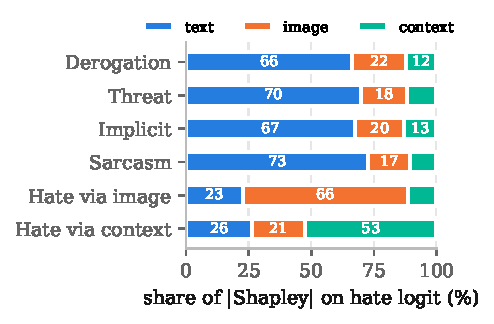
\includegraphics[width=0.88\columnwidth]{../figures/modality_shapley}
\caption{Share of absolute Shapley value on the hate logit by modality for posts predicted hateful, by functionality (GRPO policy).}
\label{fig:shap}
\end{figure}
Figure~\ref{fig:shap} shows that the policy relies on the right modality where the benchmark requires it: for hate-via-image 66\% of attribution goes to the image, for hate-via-context 53\% to the context,
while ordinary hateful text is explained by the text (66--73\%). The non-hateful rows of the figure are the (few) false positives; for the two flagged benign-context posts the image carries 74\% of the attribution, which hints that
visual cues contribute to some errors (very small $n$). The explanation report turns these numbers into statements such as
``the decision is driven mainly by the image, not by the words alone'' (Figure~\ref{fig:cases} shows token attributions for four cases).

\begin{figure*}[t]
\centering
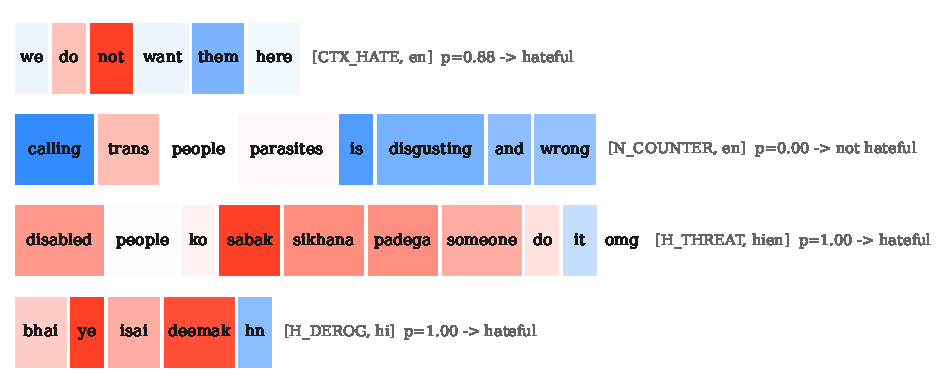
\includegraphics[width=0.78\textwidth]{../figures/case_heatmaps}
\caption{Integrated-Gradients attributions on four test posts (red: toward ``hateful''; blue: toward ``not hateful''). In the counter-speech case
\emph{wrong} and \emph{disgusting} push strongly toward ``not hateful'', while the hateful vocabulary itself receives almost no weight. In the context case, \emph{not} is the dominant token, which is a plausible
shortcut rather than the full evidence.}
\label{fig:cases}
\end{figure*}

\subsection{Low-resource transfer}
\begin{figure}[t]
\centering
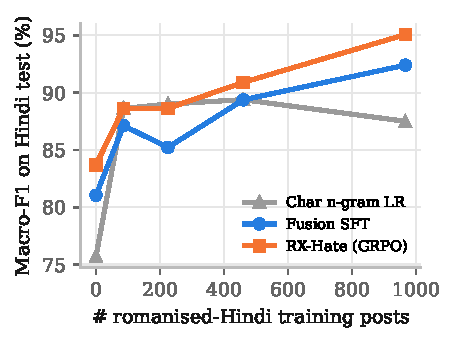
\includegraphics[width=0.78\columnwidth]{../figures/lowres}
\caption{Macro-F1 on romanised-Hindi test posts as the number of Hindi training posts grows (single seed).}
\label{fig:lowres}
\end{figure}
We vary how many romanised-Hindi posts are in the training data (0, 86, 225, 460 and 967; the English and Hinglish data stay fixed). With no Hindi training data the fusion policy reaches 81.1 F1 on Hindi test posts
(83.7 after GRPO) against 75.7 for a character-n-gram LR, showing transfer through shared sub-word features and shared identity terms. With 86--225 Hindi posts the character LR is competitive or better (88.6--89.0
vs.\ 85.2--87.1 for SFT and 88.6 for GRPO), and only with the full 967 posts do the fusion policy (92.4) and GRPO (95.1) clearly pull ahead of it (87.5). This was run with a single seed, and Hindi and Hinglish templates overlap in
vocabulary, so the analysis supports only a modest claim: GRPO is better than SFT at every Hindi training size (by 1.5--3.4 points), and ties or trails the character LR at 86 and 225 posts; it does not show robust cross-lingual transfer.

\subsection{How many human rationales are needed?}
\begin{figure}[t]
\centering
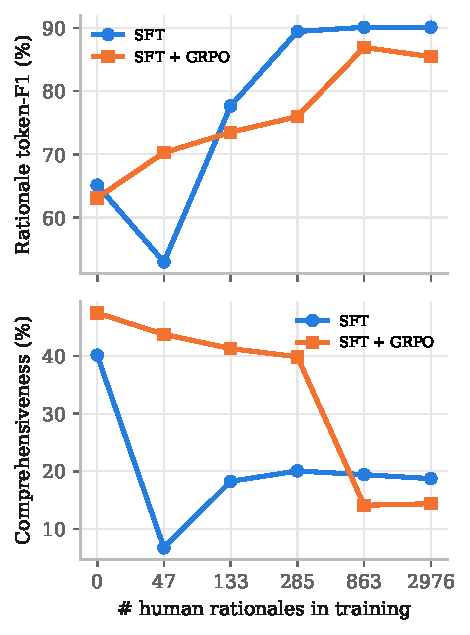
\includegraphics[width=0.85\columnwidth]{../figures/feedback}
\caption{Effect of the number of human rationales available for SFT (single seed). With 0 rationales the SFT head is untrained and highlights the whole post.}
\label{fig:fb}
\end{figure}
Figure~\ref{fig:fb} varies the number of hateful training posts with a human rationale (0 to 2{,}976). With 47 rationales, SFT overfits and its rationales are short (19.5\% of tokens) and unfaithful
(comprehensiveness 6.7), whereas GRPO recovers a token-F1 of 70.3 and comprehensiveness of 43.8. With zero rationales the SFT head is untrained and highlights the whole post; GRPO, driven only by the sparsity and faithfulness
rewards, selects 65\% of the tokens, with token-F1 63.1, which is no better than the trivial ``highlight everything'' baseline (65.1). So the reward alone does not rediscover human-like rationales, but when annotations are scarce it
keeps rationales faithful. With 863 or more rationales SFT is more plausible (about 90 vs.\ 85--87 token-F1), and in this single-seed run GRPO's comprehensiveness (14) is below SFT's (19), unlike the three-seed mean of Table~\ref{tab:abl},
which again shows how seed-dependent the faithfulness gain is. Classification F1 after GRPO stays between 85.1 and 85.8 across all budgets.

%% ---------------------------------------------------------------------------------------------
\section{LLM Instantiation (Implemented, Not Evaluated)}
The same reward functions drive an instruction-tuned LLM. The released code prompts Qwen2.5 \citep{qwen2024qwen25} with the post, the parent post and an image caption, and asks for a JSON answer
(\texttt{label}, \texttt{target}, \texttt{rationale} words copied from the post, \texttt{explanation}). It runs an SFT warm-up with LoRA \citep{hu2022lora} and GRPO with TRL \citep{vonwerra2020trl}.
Rewards are wrappers of Section~\ref{sec:reward}: format validity, correctness, identity false-positive penalty, plausibility, rationale shape (sparsity, no evidence for non-hateful answers, and a penalty for rationale words absent from the post), and faithfulness measured with a frozen judge on
the rationale-only and rationale-removed text. Reward wrappers and the answer parser are covered by unit tests; training and evaluation require a GPU and were \emph{not} run for this paper. We make no claim about the
LLM's accuracy; since LLM rationales are generated text, comparing their faithfulness against a frozen judge, as we did for the fusion policy, is the key experiment to run.

%% ---------------------------------------------------------------------------------------------
\section{Conclusion}
We cast hate-speech moderation as reward optimisation over labels and rationales and studied it on a controlled multimodal, code-mixed benchmark. GRPO with counterfactual pairing yields a modest, consistent accuracy gain over
supervised training, clearly lower identity-swap sensitivity, and explanations that identify the modality that decides a case; the faithfulness reward helps, but the resulting gain over SFT varies with the seed. The study also yields negative findings:
a strong linear baseline matches the policy's accuracy, the plausibility reward is inert, faithfulness costs human-likeness, and counter-speech remains hard for all models. The next steps are
evaluation on HateXplain, HASOC and Hateful Memes with a CLIP encoder and the LLM path, human evaluation of the explanations, and tuning of the reward weights on real data.

\section*{Limitations}
\textbf{Synthetic data.} \textsc{SynHateMM} is template-based; its difficulty and its linguistic variety are far below those of real social media, and its rationales are exact by construction.
Conclusions about rankings of methods may not transfer. \textbf{Small model.} The fusion policy uses hashed n-grams and hand-crafted image features; we did not evaluate pre-trained multilingual encoders, CLIP or LLMs. \textbf{Self-measured faithfulness.}
The faithfulness reward and the faithfulness metric both use the policy's own probabilities, so the policy may learn to satisfy the measure without a deeper notion of faithfulness; the post-hoc explainers help but are also model-based.
\textbf{Statistics.} Three seeds for the main and ablation results, a single seed for the low-resource and rationale-budget curves; no significance tests; some ablation differences (e.g.\ the fairness reward) are within one standard deviation.
\textbf{Weights and design.} Reward weights were chosen once and not tuned; the rationale is token-level and cannot express implicit, image-only evidence. \textbf{Language coverage.} Only English, Hinglish and romanised Hindi (no Devanagari script) are covered.

\section*{Ethics Statement}
Hate speech detection can both protect and harm. False positives suppress legitimate speech, including counter-speech and speech by affected communities; false negatives leave users exposed. We therefore measure identity-term bias explicitly
and report that benign identity mentions are still flagged 18\% of the time. The system is intended as decision support with the explanation shown to a human moderator, not as an automatic removal tool. The synthetic benchmark contains no slurs or real
hate symbols and was designed to avoid harm; real hate speech corpora should only be used under their licences and with ethics review. Definitions of hate speech depend on culture and law, and the rewards reflect one such definition.

\bibliography{references}

\appendix
\section{Reproducibility}
Code, configuration and the experiment script are in the accompanying repository (\texttt{scripts/run\_experiments.py} regenerates every table and figure; \texttt{scripts/make\_report.py} builds them).
Model sizes: $2^{15}$ hashed text features, hidden sizes 128 (text), 48 (image), 48 (context) and 64 (fusion). SFT: Adam, learning rate $2\cdot10^{-3}$, batch 64, dropout 0.2, modality dropout 0.15, rationale loss weight 1, patience 3.
GRPO: group size 8, clip 0.2, $\beta{=}0.04$, $\lambda{=}0.5$, learning rate $5\cdot10^{-4}$, 3 epochs, batch 32, 2 inner steps. Seeds 0--2 for model initialisation and sampling; the dataset is generated with seed 13.

\end{document}
